\section{ХОД РАБОТЫ}

\subsection{Текст задания}

Для всех вариантов необходимо выполнить следующее:

\begin{itemize}
\item
  функции, определенные в работах 4 и 5, оформить в виде библиотеки DLL;
\item
  создать новый проект для демонстрации работы с DLL и функциями;
\item
  в нечетных номерах заданий необходимо использовать
  статическое связывание с импортом; 
\item
  создать специальный заголовочный файл с объявлениями функций,
  подлежащих импорту.
\end{itemize}

\subsection{Исходные данные}

На рисунке~\ref{lst:struct_and_functions} представлена структура Complex
и ряд функций по работе с комплексными числами,
реализованных в предыдущих лабораторных работах.

\begin{lstlisting}[caption=Структура Complex
  и прототипы функций для работы с ней,
  label=lst:struct_and_functions]
 struct Complex {
   double re;
   double im;
 };
 
 struct Complex add(struct Complex c1, struct Complex c2);
 struct Complex sub(struct Complex c1, struct Complex c2);
 struct Complex mul(struct Complex c1, struct Complex c2);
 struct Complex div(struct Complex c1, struct Complex c2);
 
 void print_complex(struct Complex c);
 
 void
 writeComplex(char *fname, struct Complex *complex, int count);

 int
 readComplex(char *fname, struct Complex *complex, int count);
\end{lstlisting}

\subsection{Создание и использование динамических библиотек
  в среде \\ разработки Microsoft Visual Studio}

В этом подразделе приведено пошаговое описание действий для создания и использования
динамических библиотек в среде разработки Microsoft Visual Studio.

\paragraph{}
Создание проекта библиотеки динамической компоновки (DLL) выполняется следующим образом:
\begin{enumerate}
\item
  В меню <<Файл>> выбрать пункты <<Создать>>, <<Проект>>.
\item
  В левой области в категории <<Visual C++>> выбрать <<Win32>>.
\item
  В центральной области выбрать <<Консольное приложение Win32>>.
\item
  Указать имя для проекта --- например, MathFuncsDll --- в поле <<Имя>>.
  Указать имя для решения --- например, DynamicLibrary --- в поле <<Имя решения>>.
  Нажмите кнопку <<ОК>>.
\item
  На странице <<Обзор>> диалогового окна <<Мастер приложений Win32>> нажать кнопку <<Далее>>.
\item
  На странице <<Параметры приложения>> в разделе <<Тип приложения>> выбрать <<DLL>>.
\item
  Нажать кнопку <<Готово>>, чтобы создать проект.
\end{enumerate}

\paragraph{}
Создание консольного проекта, ссылающегося на DLL в среде
Microsoft Visual Studio выполняется следующим образом:

\begin{enumerate}
\item
  В левой области в категории <<Visual C++>> выбрать <<Win32>>.
\item
  В центральной области выбрать <<Консольное приложение Win32>>.
\item
  Указать имя проекта --- например, MyExecRefsDll --- в поле <<Имя>>.
  В раскрывающемся списке рядом с полем <<Решение>> выбрать <<Добавить в решение>>.
  В результате новый проект будет добавлен в решение, содержащее статическую библиотеку.
  Нажать кнопку <<ОК>>.
\item
  На странице <<Обзор диалогового окна Мастер приложений Win32>> нажать кнопку <<Далее>>.
\item
  На странице <<Параметры приложения>> выбрать в поле <<Тип приложения>> пункт
  <<Консольное приложение>>.
\item
  На странице <<Параметры приложения>> в разделе <<Дополнительные параметры>>
  снять флажок <<Предкомпилированный заголовок>>.
\item
  Нажать кнопку <<Готово>>, чтобы создать проект.
\end{enumerate}

Для того, чтобы использовать функциональность статической библиотеки в проекте
Microsoft Visual Studio, следует выполнить следующие операции:

\begin{enumerate}
\item
  Открыть контекстное меню проекта MyExecRefsLib в области
  <<Обозреватель решений>> и выбрать <<Ссылки>>.
\item
  В диалоговом окне <<Страницы свойств MyExecRefsLib>> развернуть узел <<Общие свойства>>,
  выбрать <<.NET Framework и ссылки>> и нажать кнопку <<Добавить новую ссылку>>.
\item
  Установить флажок рядом с MathFuncsLib на вкладке <<Проекты>>,
  а затем нажать кнопку <<ОК>>.
\item
  Для создания ссылки на файл заголовка MathFuncsLib.h необходимо изменить путь
  к каталогам включения.
  Для этого в диалоговом окне Окна свойств библиотеки MyExecRefsLib последовательно
  развернуть узлы <<Свойства конфигурации>>, <<C/C++>>, затем выбрать <<Общие>>.
  В поле <<Дополнительные каталоги включаемых файлов>> указать путь к каталогу
  MathFuncsLib.
\item
  Нажать кнопку <<ОК>> для сохранения изменений в проект.
\end{enumerate}

\pagebreak 

\subsection{Особенности разработанной программы}
\label{ssec:program_description}

В ходе проведения данной лабораторной работы была проведена реорганизация 
исходных файлов проекта, преследующая следующие цели:

\begin{itemize}
\item уменьшение числа зависимостей в файлах с исходным кодом;
\item выделение кода функций, выполняющих обработку структуры Complex, 
  в отдельные библиотеки.
\end{itemize}

Схема зависимостей исходных файлов проекта показана на рисунке~\ref{fig:dependencies}.

\begin{figure}[htbp]
  \centering
  \small{
    % Graphic for TeX using PGF
% Title: /home/budnyjj/univer/GIT/discipline/SPO/lab_6/report/img/dependencies.dia
% Creator: Dia v0.97.2
% CreationDate: Sat May  3 14:50:51 2014
% For: budnyjj
% \usepackage{tikz}
% The following commands are not supported in PSTricks at present
% We define them conditionally, so when they are implemented,
% this pgf file will use them.
\ifx\du\undefined
  \newlength{\du}
\fi
\setlength{\du}{15\unitlength}
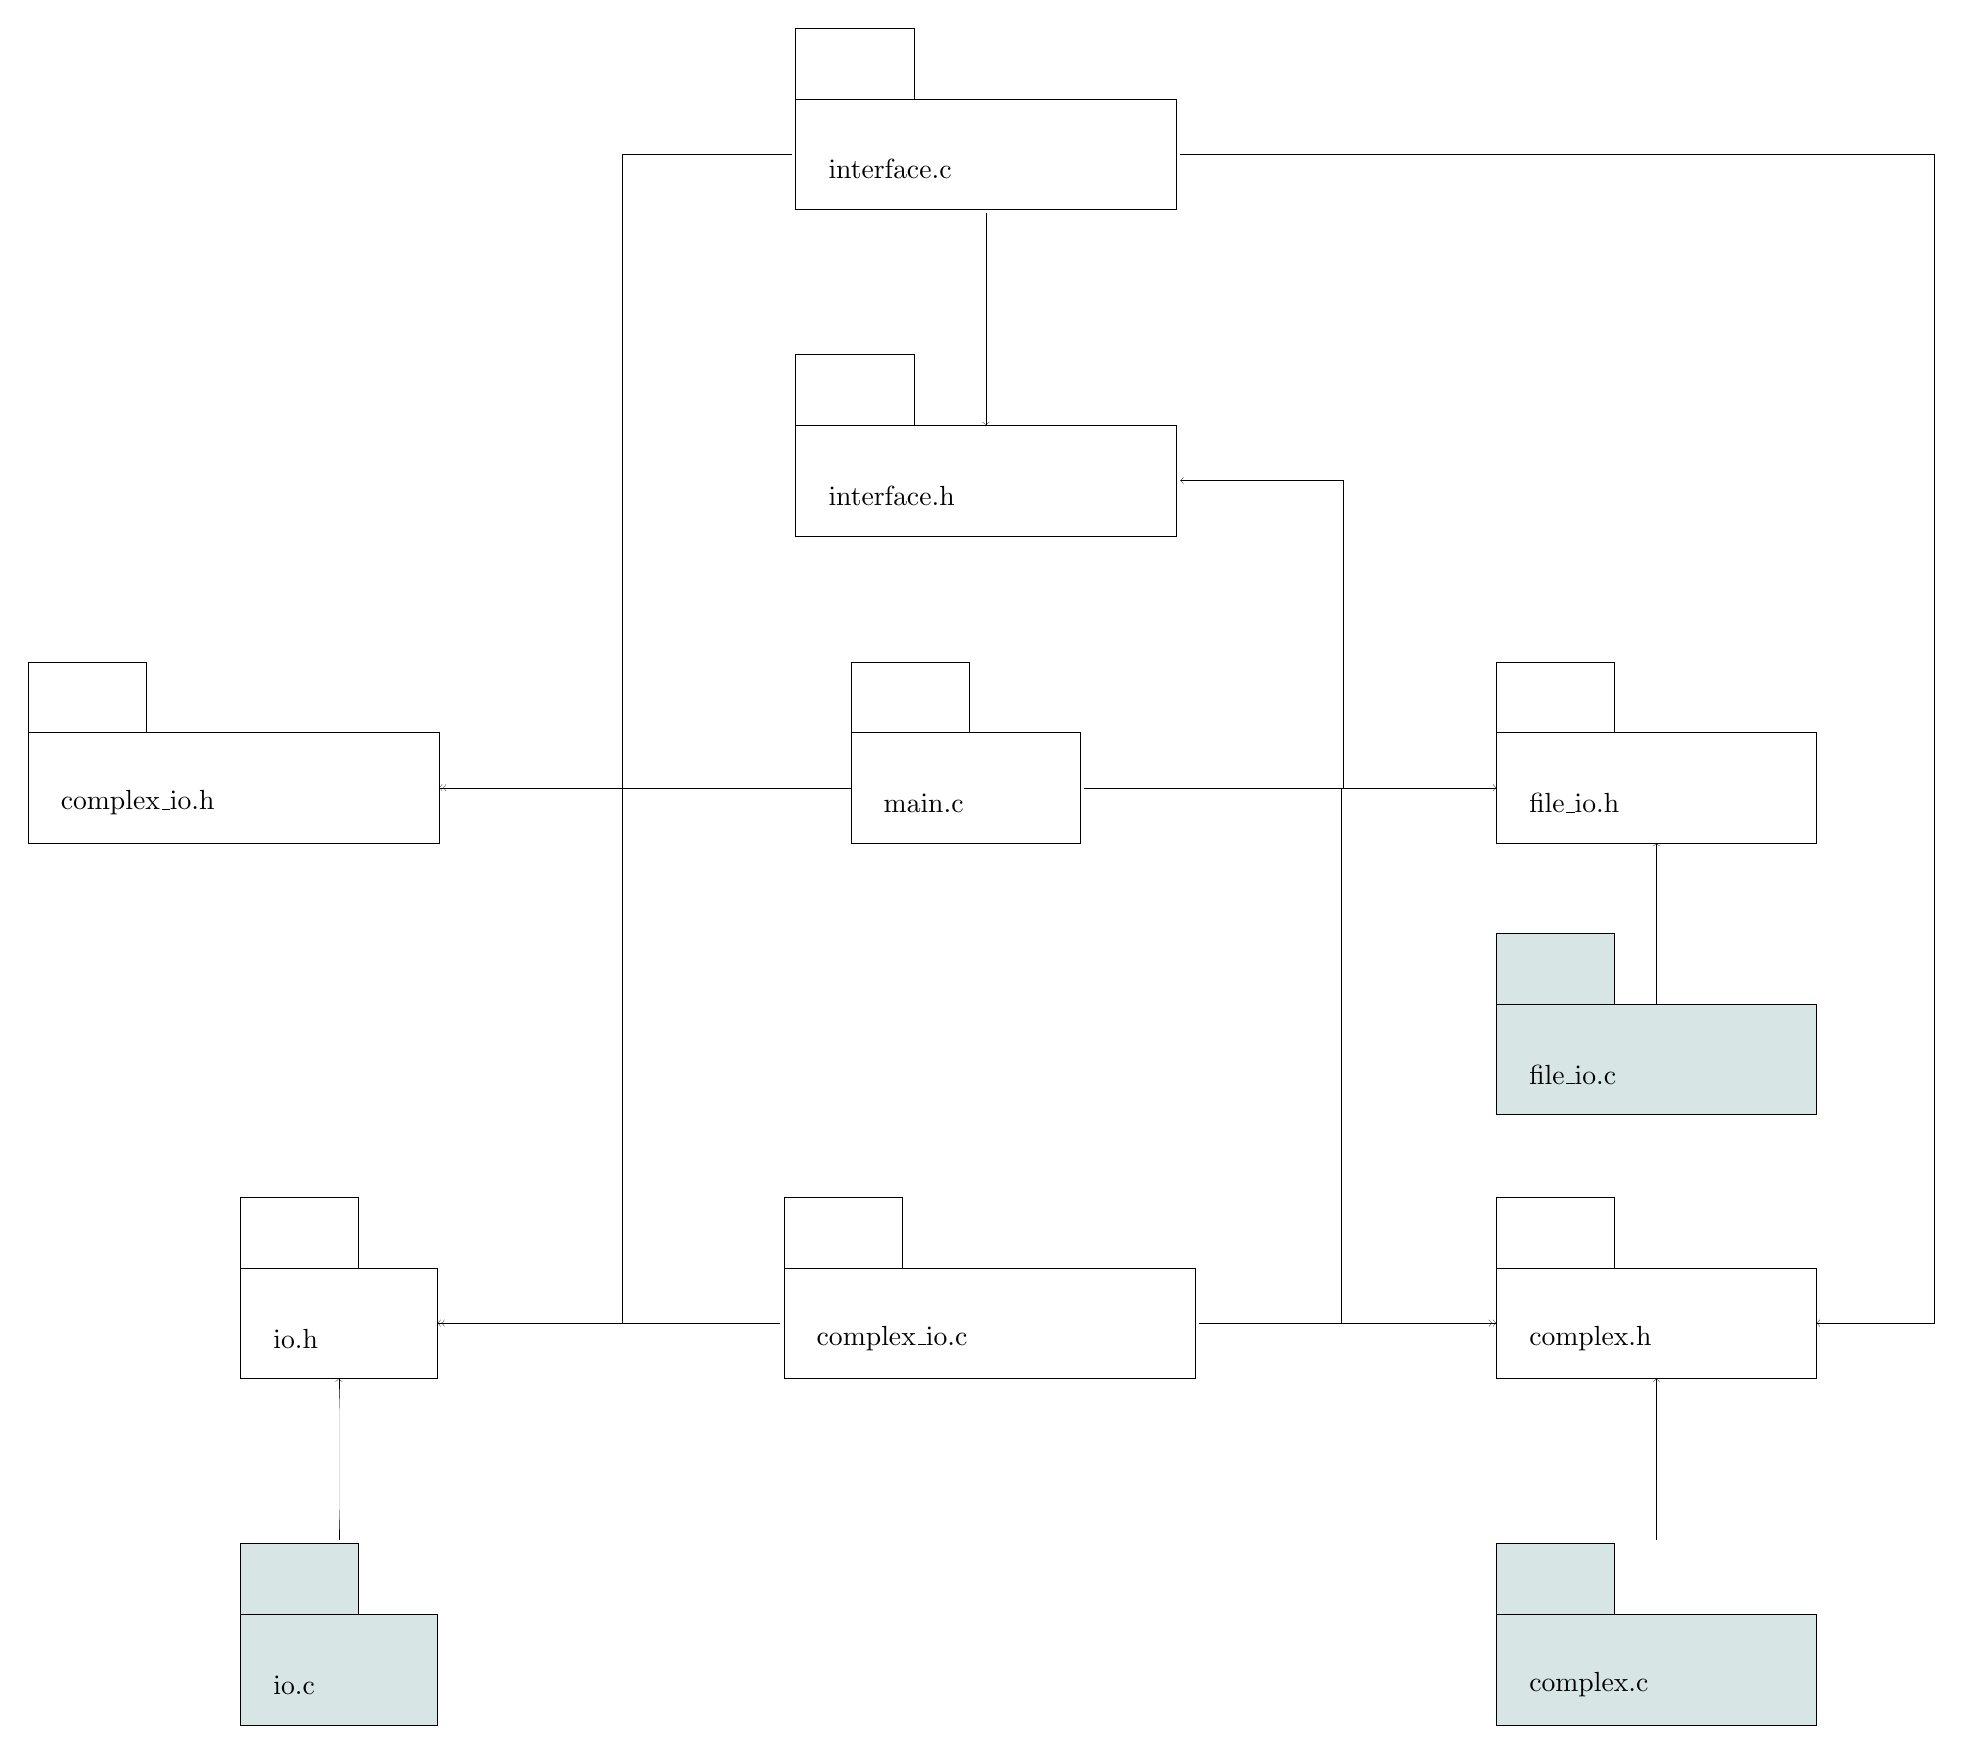
\begin{tikzpicture}
\pgftransformxscale{1.000000}
\pgftransformyscale{-1.000000}
\definecolor{dialinecolor}{rgb}{0.000000, 0.000000, 0.000000}
\pgfsetstrokecolor{dialinecolor}
\definecolor{dialinecolor}{rgb}{1.000000, 1.000000, 1.000000}
\pgfsetfillcolor{dialinecolor}
\pgfsetlinewidth{0.100000\du}
\pgfsetdash{}{0pt}
\definecolor{dialinecolor}{rgb}{1.000000, 1.000000, 1.000000}
\pgfsetfillcolor{dialinecolor}
\fill (36.000000\du,33.400000\du)--(36.000000\du,34.800000\du)--(40.065000\du,34.800000\du)--(40.065000\du,33.400000\du)--cycle;
\definecolor{dialinecolor}{rgb}{0.000000, 0.000000, 0.000000}
\pgfsetstrokecolor{dialinecolor}
\draw (36.000000\du,33.400000\du)--(36.000000\du,34.800000\du)--(40.065000\du,34.800000\du)--(40.065000\du,33.400000\du)--cycle;
\definecolor{dialinecolor}{rgb}{1.000000, 1.000000, 1.000000}
\pgfsetfillcolor{dialinecolor}
\fill (36.000000\du,32.500000\du)--(36.000000\du,33.400000\du)--(37.500000\du,33.400000\du)--(37.500000\du,32.500000\du)--cycle;
\definecolor{dialinecolor}{rgb}{0.000000, 0.000000, 0.000000}
\pgfsetstrokecolor{dialinecolor}
\draw (36.000000\du,32.500000\du)--(36.000000\du,33.400000\du)--(37.500000\du,33.400000\du)--(37.500000\du,32.500000\du)--cycle;
% setfont left to latex
\definecolor{dialinecolor}{rgb}{0.000000, 0.000000, 0.000000}
\pgfsetstrokecolor{dialinecolor}
\node[anchor=west] at (36.300000\du,34.295000\du){complex.h};
\pgfsetlinewidth{0.100000\du}
\pgfsetdash{}{0pt}
\definecolor{dialinecolor}{rgb}{1.000000, 1.000000, 1.000000}
\pgfsetfillcolor{dialinecolor}
\fill (17.350000\du,26.600000\du)--(17.350000\du,28.000000\du)--(22.570000\du,28.000000\du)--(22.570000\du,26.600000\du)--cycle;
\definecolor{dialinecolor}{rgb}{0.000000, 0.000000, 0.000000}
\pgfsetstrokecolor{dialinecolor}
\draw (17.350000\du,26.600000\du)--(17.350000\du,28.000000\du)--(22.570000\du,28.000000\du)--(22.570000\du,26.600000\du)--cycle;
\definecolor{dialinecolor}{rgb}{1.000000, 1.000000, 1.000000}
\pgfsetfillcolor{dialinecolor}
\fill (17.350000\du,25.700000\du)--(17.350000\du,26.600000\du)--(18.850000\du,26.600000\du)--(18.850000\du,25.700000\du)--cycle;
\definecolor{dialinecolor}{rgb}{0.000000, 0.000000, 0.000000}
\pgfsetstrokecolor{dialinecolor}
\draw (17.350000\du,25.700000\du)--(17.350000\du,26.600000\du)--(18.850000\du,26.600000\du)--(18.850000\du,25.700000\du)--cycle;
% setfont left to latex
\definecolor{dialinecolor}{rgb}{0.000000, 0.000000, 0.000000}
\pgfsetstrokecolor{dialinecolor}
\node[anchor=west] at (17.650000\du,27.495000\du){complex\_io.h};
\pgfsetlinewidth{0.100000\du}
\pgfsetdash{}{0pt}
\definecolor{dialinecolor}{rgb}{1.000000, 1.000000, 1.000000}
\pgfsetfillcolor{dialinecolor}
\fill (36.000000\du,26.600000\du)--(36.000000\du,28.000000\du)--(40.065000\du,28.000000\du)--(40.065000\du,26.600000\du)--cycle;
\definecolor{dialinecolor}{rgb}{0.000000, 0.000000, 0.000000}
\pgfsetstrokecolor{dialinecolor}
\draw (36.000000\du,26.600000\du)--(36.000000\du,28.000000\du)--(40.065000\du,28.000000\du)--(40.065000\du,26.600000\du)--cycle;
\definecolor{dialinecolor}{rgb}{1.000000, 1.000000, 1.000000}
\pgfsetfillcolor{dialinecolor}
\fill (36.000000\du,25.700000\du)--(36.000000\du,26.600000\du)--(37.500000\du,26.600000\du)--(37.500000\du,25.700000\du)--cycle;
\definecolor{dialinecolor}{rgb}{0.000000, 0.000000, 0.000000}
\pgfsetstrokecolor{dialinecolor}
\draw (36.000000\du,25.700000\du)--(36.000000\du,26.600000\du)--(37.500000\du,26.600000\du)--(37.500000\du,25.700000\du)--cycle;
% setfont left to latex
\definecolor{dialinecolor}{rgb}{0.000000, 0.000000, 0.000000}
\pgfsetstrokecolor{dialinecolor}
\node[anchor=west] at (36.300000\du,27.495000\du){file\_io.h};
\pgfsetlinewidth{0.100000\du}
\pgfsetdash{}{0pt}
\definecolor{dialinecolor}{rgb}{1.000000, 1.000000, 1.000000}
\pgfsetfillcolor{dialinecolor}
\fill (27.100000\du,22.700000\du)--(27.100000\du,24.100000\du)--(31.935000\du,24.100000\du)--(31.935000\du,22.700000\du)--cycle;
\definecolor{dialinecolor}{rgb}{0.000000, 0.000000, 0.000000}
\pgfsetstrokecolor{dialinecolor}
\draw (27.100000\du,22.700000\du)--(27.100000\du,24.100000\du)--(31.935000\du,24.100000\du)--(31.935000\du,22.700000\du)--cycle;
\definecolor{dialinecolor}{rgb}{1.000000, 1.000000, 1.000000}
\pgfsetfillcolor{dialinecolor}
\fill (27.100000\du,21.800000\du)--(27.100000\du,22.700000\du)--(28.600000\du,22.700000\du)--(28.600000\du,21.800000\du)--cycle;
\definecolor{dialinecolor}{rgb}{0.000000, 0.000000, 0.000000}
\pgfsetstrokecolor{dialinecolor}
\draw (27.100000\du,21.800000\du)--(27.100000\du,22.700000\du)--(28.600000\du,22.700000\du)--(28.600000\du,21.800000\du)--cycle;
% setfont left to latex
\definecolor{dialinecolor}{rgb}{0.000000, 0.000000, 0.000000}
\pgfsetstrokecolor{dialinecolor}
\node[anchor=west] at (27.400000\du,23.595000\du){interface.h};
\pgfsetlinewidth{0.100000\du}
\pgfsetdash{}{0pt}
\definecolor{dialinecolor}{rgb}{1.000000, 1.000000, 1.000000}
\pgfsetfillcolor{dialinecolor}
\fill (20.050000\du,33.400000\du)--(20.050000\du,34.800000\du)--(22.550000\du,34.800000\du)--(22.550000\du,33.400000\du)--cycle;
\definecolor{dialinecolor}{rgb}{0.000000, 0.000000, 0.000000}
\pgfsetstrokecolor{dialinecolor}
\draw (20.050000\du,33.400000\du)--(20.050000\du,34.800000\du)--(22.550000\du,34.800000\du)--(22.550000\du,33.400000\du)--cycle;
\definecolor{dialinecolor}{rgb}{1.000000, 1.000000, 1.000000}
\pgfsetfillcolor{dialinecolor}
\fill (20.050000\du,32.500000\du)--(20.050000\du,33.400000\du)--(21.550000\du,33.400000\du)--(21.550000\du,32.500000\du)--cycle;
\definecolor{dialinecolor}{rgb}{0.000000, 0.000000, 0.000000}
\pgfsetstrokecolor{dialinecolor}
\draw (20.050000\du,32.500000\du)--(20.050000\du,33.400000\du)--(21.550000\du,33.400000\du)--(21.550000\du,32.500000\du)--cycle;
% setfont left to latex
\definecolor{dialinecolor}{rgb}{0.000000, 0.000000, 0.000000}
\pgfsetstrokecolor{dialinecolor}
\node[anchor=west] at (20.350000\du,34.295000\du){io.h};
\pgfsetlinewidth{0.100000\du}
\pgfsetdash{}{0pt}
\definecolor{dialinecolor}{rgb}{1.000000, 1.000000, 1.000000}
\pgfsetfillcolor{dialinecolor}
\fill (26.950000\du,33.400000\du)--(26.950000\du,34.800000\du)--(32.170000\du,34.800000\du)--(32.170000\du,33.400000\du)--cycle;
\definecolor{dialinecolor}{rgb}{0.000000, 0.000000, 0.000000}
\pgfsetstrokecolor{dialinecolor}
\draw (26.950000\du,33.400000\du)--(26.950000\du,34.800000\du)--(32.170000\du,34.800000\du)--(32.170000\du,33.400000\du)--cycle;
\definecolor{dialinecolor}{rgb}{1.000000, 1.000000, 1.000000}
\pgfsetfillcolor{dialinecolor}
\fill (26.950000\du,32.500000\du)--(26.950000\du,33.400000\du)--(28.450000\du,33.400000\du)--(28.450000\du,32.500000\du)--cycle;
\definecolor{dialinecolor}{rgb}{0.000000, 0.000000, 0.000000}
\pgfsetstrokecolor{dialinecolor}
\draw (26.950000\du,32.500000\du)--(26.950000\du,33.400000\du)--(28.450000\du,33.400000\du)--(28.450000\du,32.500000\du)--cycle;
% setfont left to latex
\definecolor{dialinecolor}{rgb}{0.000000, 0.000000, 0.000000}
\pgfsetstrokecolor{dialinecolor}
\node[anchor=west] at (27.250000\du,34.295000\du){complex\_io.c};
\pgfsetlinewidth{0.100000\du}
\pgfsetdash{}{0pt}
\definecolor{dialinecolor}{rgb}{1.000000, 1.000000, 1.000000}
\pgfsetfillcolor{dialinecolor}
\fill (27.800000\du,26.600000\du)--(27.800000\du,28.000000\du)--(30.710000\du,28.000000\du)--(30.710000\du,26.600000\du)--cycle;
\definecolor{dialinecolor}{rgb}{0.000000, 0.000000, 0.000000}
\pgfsetstrokecolor{dialinecolor}
\draw (27.800000\du,26.600000\du)--(27.800000\du,28.000000\du)--(30.710000\du,28.000000\du)--(30.710000\du,26.600000\du)--cycle;
\definecolor{dialinecolor}{rgb}{1.000000, 1.000000, 1.000000}
\pgfsetfillcolor{dialinecolor}
\fill (27.800000\du,25.700000\du)--(27.800000\du,26.600000\du)--(29.300000\du,26.600000\du)--(29.300000\du,25.700000\du)--cycle;
\definecolor{dialinecolor}{rgb}{0.000000, 0.000000, 0.000000}
\pgfsetstrokecolor{dialinecolor}
\draw (27.800000\du,25.700000\du)--(27.800000\du,26.600000\du)--(29.300000\du,26.600000\du)--(29.300000\du,25.700000\du)--cycle;
% setfont left to latex
\definecolor{dialinecolor}{rgb}{0.000000, 0.000000, 0.000000}
\pgfsetstrokecolor{dialinecolor}
\node[anchor=west] at (28.100000\du,27.495000\du){main.c};
\pgfsetlinewidth{0.100000\du}
\pgfsetbuttcap
\pgfsetdash{}{0pt}
{
\definecolor{dialinecolor}{rgb}{0.000000, 0.000000, 0.000000}
\pgfsetfillcolor{dialinecolor}
% was here!!!
\pgfsetarrowsend{to}
\definecolor{dialinecolor}{rgb}{0.000000, 0.000000, 0.000000}
\pgfsetstrokecolor{dialinecolor}
\draw (27.753716\du,27.300000\du)--(24.900000\du,27.300000\du)--(24.900000\du,34.100000\du)--(22.550000\du,34.100000\du);
}
% setfont left to latex
\pgfsetlinewidth{0.100000\du}
\pgfsetbuttcap
\pgfsetdash{}{0pt}
{
\definecolor{dialinecolor}{rgb}{0.000000, 0.000000, 0.000000}
\pgfsetfillcolor{dialinecolor}
% was here!!!
\pgfsetarrowsend{to}
\definecolor{dialinecolor}{rgb}{0.000000, 0.000000, 0.000000}
\pgfsetstrokecolor{dialinecolor}
\draw (30.759486\du,27.300000\du)--(34.030184\du,27.300000\du)--(34.030184\du,34.100000\du)--(36.000000\du,34.100000\du);
}
% setfont left to latex
\pgfsetlinewidth{0.100000\du}
\pgfsetbuttcap
\pgfsetdash{}{0pt}
{
\definecolor{dialinecolor}{rgb}{0.000000, 0.000000, 0.000000}
\pgfsetfillcolor{dialinecolor}
% was here!!!
\pgfsetarrowsend{to}
\definecolor{dialinecolor}{rgb}{0.000000, 0.000000, 0.000000}
\pgfsetstrokecolor{dialinecolor}
\draw (30.760367\du,27.300000\du)--(31.260367\du,27.300000\du)--(35.500000\du,27.300000\du)--(36.000000\du,27.300000\du);
}
% setfont left to latex
\pgfsetlinewidth{0.100000\du}
\pgfsetbuttcap
\pgfsetdash{}{0pt}
{
\definecolor{dialinecolor}{rgb}{0.000000, 0.000000, 0.000000}
\pgfsetfillcolor{dialinecolor}
% was here!!!
\pgfsetarrowsend{to}
\definecolor{dialinecolor}{rgb}{0.000000, 0.000000, 0.000000}
\pgfsetstrokecolor{dialinecolor}
\draw (27.800000\du,27.300000\du)--(27.300000\du,27.300000\du)--(23.070000\du,27.300000\du)--(22.570000\du,27.300000\du);
}
% setfont left to latex
\pgfsetlinewidth{0.100000\du}
\pgfsetbuttcap
\pgfsetdash{}{0pt}
{
\definecolor{dialinecolor}{rgb}{0.000000, 0.000000, 0.000000}
\pgfsetfillcolor{dialinecolor}
% was here!!!
\pgfsetarrowsend{to}
\definecolor{dialinecolor}{rgb}{0.000000, 0.000000, 0.000000}
\pgfsetstrokecolor{dialinecolor}
\draw (30.759291\du,27.300000\du)--(34.050000\du,27.300000\du)--(34.050000\du,23.400000\du)--(31.984039\du,23.400000\du);
}
% setfont left to latex
\pgfsetlinewidth{0.100000\du}
\pgfsetbuttcap
\pgfsetdash{}{0pt}
{
\definecolor{dialinecolor}{rgb}{0.000000, 0.000000, 0.000000}
\pgfsetfillcolor{dialinecolor}
% was here!!!
\pgfsetarrowsend{to}
\definecolor{dialinecolor}{rgb}{0.000000, 0.000000, 0.000000}
\pgfsetstrokecolor{dialinecolor}
\draw (26.899675\du,34.100000\du)--(26.399675\du,34.100000\du)--(23.100317\du,34.100000\du)--(22.600317\du,34.100000\du);
}
% setfont left to latex
\pgfsetlinewidth{0.100000\du}
\pgfsetbuttcap
\pgfsetdash{}{0pt}
{
\definecolor{dialinecolor}{rgb}{0.000000, 0.000000, 0.000000}
\pgfsetfillcolor{dialinecolor}
% was here!!!
\pgfsetarrowsend{to}
\definecolor{dialinecolor}{rgb}{0.000000, 0.000000, 0.000000}
\pgfsetstrokecolor{dialinecolor}
\draw (32.220325\du,34.100000\du)--(32.720325\du,34.100000\du)--(35.449746\du,34.100000\du)--(35.949746\du,34.100000\du);
}
% setfont left to latex
\pgfsetlinewidth{0.100000\du}
\pgfsetdash{}{0pt}
\definecolor{dialinecolor}{rgb}{1.000000, 1.000000, 1.000000}
\pgfsetfillcolor{dialinecolor}
\fill (27.100000\du,18.550000\du)--(27.100000\du,19.950000\du)--(31.935000\du,19.950000\du)--(31.935000\du,18.550000\du)--cycle;
\definecolor{dialinecolor}{rgb}{0.000000, 0.000000, 0.000000}
\pgfsetstrokecolor{dialinecolor}
\draw (27.100000\du,18.550000\du)--(27.100000\du,19.950000\du)--(31.935000\du,19.950000\du)--(31.935000\du,18.550000\du)--cycle;
\definecolor{dialinecolor}{rgb}{1.000000, 1.000000, 1.000000}
\pgfsetfillcolor{dialinecolor}
\fill (27.100000\du,17.650000\du)--(27.100000\du,18.550000\du)--(28.600000\du,18.550000\du)--(28.600000\du,17.650000\du)--cycle;
\definecolor{dialinecolor}{rgb}{0.000000, 0.000000, 0.000000}
\pgfsetstrokecolor{dialinecolor}
\draw (27.100000\du,17.650000\du)--(27.100000\du,18.550000\du)--(28.600000\du,18.550000\du)--(28.600000\du,17.650000\du)--cycle;
% setfont left to latex
\definecolor{dialinecolor}{rgb}{0.000000, 0.000000, 0.000000}
\pgfsetstrokecolor{dialinecolor}
\node[anchor=west] at (27.400000\du,19.445000\du){interface.c};
\pgfsetlinewidth{0.100000\du}
\pgfsetbuttcap
\pgfsetdash{}{0pt}
{
\definecolor{dialinecolor}{rgb}{0.000000, 0.000000, 0.000000}
\pgfsetfillcolor{dialinecolor}
% was here!!!
\pgfsetarrowsend{to}
\definecolor{dialinecolor}{rgb}{0.000000, 0.000000, 0.000000}
\pgfsetstrokecolor{dialinecolor}
\draw (29.517500\du,20.000366\du)--(29.517500\du,20.500366\du)--(29.517500\du,22.200000\du)--(29.517500\du,22.700000\du);
}
% setfont left to latex
\pgfsetlinewidth{0.100000\du}
\pgfsetbuttcap
\pgfsetdash{}{0pt}
{
\definecolor{dialinecolor}{rgb}{0.000000, 0.000000, 0.000000}
\pgfsetfillcolor{dialinecolor}
% was here!!!
\pgfsetarrowsend{to}
\definecolor{dialinecolor}{rgb}{0.000000, 0.000000, 0.000000}
\pgfsetstrokecolor{dialinecolor}
\draw (27.050362\du,19.250000\du)--(24.900000\du,19.250000\du)--(24.900000\du,27.300000\du)--(22.619351\du,27.300000\du);
}
% setfont left to latex
\pgfsetlinewidth{0.100000\du}
\pgfsetbuttcap
\pgfsetdash{}{0pt}
{
\definecolor{dialinecolor}{rgb}{0.000000, 0.000000, 0.000000}
\pgfsetfillcolor{dialinecolor}
% was here!!!
\pgfsetarrowsend{to}
\definecolor{dialinecolor}{rgb}{0.000000, 0.000000, 0.000000}
\pgfsetstrokecolor{dialinecolor}
\draw (31.985301\du,19.250000\du)--(41.565000\du,19.250000\du)--(41.565000\du,34.100000\du)--(40.065000\du,34.100000\du);
}
% setfont left to latex
\pgfsetlinewidth{0.100000\du}
\pgfsetdash{}{0pt}
\definecolor{dialinecolor}{rgb}{0.847059, 0.898039, 0.898039}
\pgfsetfillcolor{dialinecolor}
\fill (36.000000\du,37.800000\du)--(36.000000\du,39.200000\du)--(40.065000\du,39.200000\du)--(40.065000\du,37.800000\du)--cycle;
\definecolor{dialinecolor}{rgb}{0.000000, 0.000000, 0.000000}
\pgfsetstrokecolor{dialinecolor}
\draw (36.000000\du,37.800000\du)--(36.000000\du,39.200000\du)--(40.065000\du,39.200000\du)--(40.065000\du,37.800000\du)--cycle;
\definecolor{dialinecolor}{rgb}{0.847059, 0.898039, 0.898039}
\pgfsetfillcolor{dialinecolor}
\fill (36.000000\du,36.900000\du)--(36.000000\du,37.800000\du)--(37.500000\du,37.800000\du)--(37.500000\du,36.900000\du)--cycle;
\definecolor{dialinecolor}{rgb}{0.000000, 0.000000, 0.000000}
\pgfsetstrokecolor{dialinecolor}
\draw (36.000000\du,36.900000\du)--(36.000000\du,37.800000\du)--(37.500000\du,37.800000\du)--(37.500000\du,36.900000\du)--cycle;
% setfont left to latex
\definecolor{dialinecolor}{rgb}{0.000000, 0.000000, 0.000000}
\pgfsetstrokecolor{dialinecolor}
\node[anchor=west] at (36.300000\du,38.695000\du){complex.c};
\pgfsetlinewidth{0.100000\du}
\pgfsetdash{}{0pt}
\definecolor{dialinecolor}{rgb}{0.847059, 0.898039, 0.898039}
\pgfsetfillcolor{dialinecolor}
\fill (20.050000\du,37.800000\du)--(20.050000\du,39.200000\du)--(22.550000\du,39.200000\du)--(22.550000\du,37.800000\du)--cycle;
\definecolor{dialinecolor}{rgb}{0.000000, 0.000000, 0.000000}
\pgfsetstrokecolor{dialinecolor}
\draw (20.050000\du,37.800000\du)--(20.050000\du,39.200000\du)--(22.550000\du,39.200000\du)--(22.550000\du,37.800000\du)--cycle;
\definecolor{dialinecolor}{rgb}{0.847059, 0.898039, 0.898039}
\pgfsetfillcolor{dialinecolor}
\fill (20.050000\du,36.900000\du)--(20.050000\du,37.800000\du)--(21.550000\du,37.800000\du)--(21.550000\du,36.900000\du)--cycle;
\definecolor{dialinecolor}{rgb}{0.000000, 0.000000, 0.000000}
\pgfsetstrokecolor{dialinecolor}
\draw (20.050000\du,36.900000\du)--(20.050000\du,37.800000\du)--(21.550000\du,37.800000\du)--(21.550000\du,36.900000\du)--cycle;
% setfont left to latex
\definecolor{dialinecolor}{rgb}{0.000000, 0.000000, 0.000000}
\pgfsetstrokecolor{dialinecolor}
\node[anchor=west] at (20.350000\du,38.695000\du){io.c};
\pgfsetlinewidth{0.100000\du}
\pgfsetdash{}{0pt}
\definecolor{dialinecolor}{rgb}{0.847059, 0.898039, 0.898039}
\pgfsetfillcolor{dialinecolor}
\fill (36.000000\du,30.050000\du)--(36.000000\du,31.450000\du)--(40.065000\du,31.450000\du)--(40.065000\du,30.050000\du)--cycle;
\definecolor{dialinecolor}{rgb}{0.000000, 0.000000, 0.000000}
\pgfsetstrokecolor{dialinecolor}
\draw (36.000000\du,30.050000\du)--(36.000000\du,31.450000\du)--(40.065000\du,31.450000\du)--(40.065000\du,30.050000\du)--cycle;
\definecolor{dialinecolor}{rgb}{0.847059, 0.898039, 0.898039}
\pgfsetfillcolor{dialinecolor}
\fill (36.000000\du,29.150000\du)--(36.000000\du,30.050000\du)--(37.500000\du,30.050000\du)--(37.500000\du,29.150000\du)--cycle;
\definecolor{dialinecolor}{rgb}{0.000000, 0.000000, 0.000000}
\pgfsetstrokecolor{dialinecolor}
\draw (36.000000\du,29.150000\du)--(36.000000\du,30.050000\du)--(37.500000\du,30.050000\du)--(37.500000\du,29.150000\du)--cycle;
% setfont left to latex
\definecolor{dialinecolor}{rgb}{0.000000, 0.000000, 0.000000}
\pgfsetstrokecolor{dialinecolor}
\node[anchor=west] at (36.300000\du,30.945000\du){file\_io.c};
\pgfsetlinewidth{0.100000\du}
\pgfsetbuttcap
\pgfsetdash{}{0pt}
{
\definecolor{dialinecolor}{rgb}{0.000000, 0.000000, 0.000000}
\pgfsetfillcolor{dialinecolor}
% was here!!!
\pgfsetarrowsend{to}
\definecolor{dialinecolor}{rgb}{0.000000, 0.000000, 0.000000}
\pgfsetstrokecolor{dialinecolor}
\draw (38.032500\du,36.849597\du)--(38.032500\du,36.349597\du)--(38.032500\du,35.300000\du)--(38.032500\du,34.800000\du);
}
% setfont left to latex
\pgfsetlinewidth{0.100000\du}
\pgfsetbuttcap
\pgfsetdash{}{0pt}
{
\definecolor{dialinecolor}{rgb}{0.000000, 0.000000, 0.000000}
\pgfsetfillcolor{dialinecolor}
% was here!!!
\pgfsetarrowsend{to}
\definecolor{dialinecolor}{rgb}{0.000000, 0.000000, 0.000000}
\pgfsetstrokecolor{dialinecolor}
\draw (38.032500\du,30.050000\du)--(38.032500\du,29.550000\du)--(38.032500\du,28.500000\du)--(38.032500\du,28.000000\du);
}
% setfont left to latex
\pgfsetlinewidth{0.100000\du}
\pgfsetbuttcap
\pgfsetdash{}{0pt}
{
\definecolor{dialinecolor}{rgb}{0.000000, 0.000000, 0.000000}
\pgfsetfillcolor{dialinecolor}
% was here!!!
\pgfsetarrowsend{to}
\definecolor{dialinecolor}{rgb}{0.000000, 0.000000, 0.000000}
\pgfsetstrokecolor{dialinecolor}
\draw (21.300000\du,36.849597\du)--(21.300000\du,36.349597\du)--(21.300000\du,35.300000\du)--(21.300000\du,34.800000\du);
}
% setfont left to latex
\end{tikzpicture}

  }
  \caption{Схема зависимостей исходных файлов проекта}\label{fig:dependencies}
\end{figure}

Файлы, помеченные синим цветом, компилируются в статические библиотеки,
так как они имеют зависимости только от одного файла с описаниями функций.
Каждый из этих файлов содержит определения логически-независимых операций со 
структурой Complex:

\begin{itemize}
  \item complex.c содержит функции арифметических операций над структурой типа Complex;
  \item io.c содержит вспомогательные функции для работы с консолью.
\end{itemize} 

Остальные файлы исходного кода программы имеют следующие назначения:
\begin{itemize}
  \item main.c содержит функцию main(), используемую для запуска программы;
  \item interface.c содержит функции для взаимодействия с пользователем через
    консольный интерфейс;
  \item file\_io.c содержит функции для чтения и записи Complex в файл;
  \item complex\_io.c содержит функции для ввода содержимого структуры Complex
    через консольный интерфейс.
\end{itemize}

После реорганизации исходного кода проекта была выполнена компиляция приложения.

Главное меню скомпилированного приложения показано на рисунке~\ref{fig:main_menu}.

\begin{figure}[htbp]
  \centering
  \includegraphics[width=150mm,height=80mm]{img/main_menu}
  \caption{Главное меню программы}\label{fig:main_menu}
\end{figure}

Исходный текст разработанной программы расположен в приложении~А.

\newpage